%%
%% Copyright 2007, 2008, 2009 Elsevier Ltd
%%
%% This file is part of the 'Elsarticle Bundle'.
%% ---------------------------------------------
%%
%% It may be distributed under the conditions of the LaTeX Project Public
%% License, either version 1.2 of this license or (at your option) any
%% later version.  The latest version of this license is in
%%    http://www.latex-project.org/lppl.txt
%% and version 1.2 or later is part of all distributions of LaTeX
%% version 1999/12/01 or later.
%%
%% The list of all files belonging to the 'Elsarticle Bundle' is
%% given in the file `manifest.txt'.
%%

%% Template article for Elsevier's document class `elsarticle'
%% with numbered style bibliographic references
%% SP 2008/03/01
%%
%%
%%
%% $Id: elsarticle-template-num.tex 4 2009-10-24 08:22:58Z rishi $
%%
%%
%\documentclass[preprint,12pt,3p]{elsarticle}

%% Use the option review to obtain double line spacing
%% \documentclass[preprint,review,12pt]{elsarticle}

%% Use the options 1p,twocolumn; 3p; 3p,twocolumn; 5p; or 5p,twocolumn
%% for a journal layout:
%% \documentclass[final,1p,times]{elsarticle}
%% \documentclass[final,1p,times,twocolumn]{elsarticle}
%% \documentclass[final,3p,times]{elsarticle}
\documentclass[final,3p,times,twocolumn]{elsarticle}
%% \documentclass[final,5p,times]{elsarticle}
%% \documentclass[final,5p,times,twocolumn]{elsarticle}

\usepackage{graphicx}
%% \usepackage{amsthm}
\usepackage[utf8]{inputenc}
\usepackage{textcomp,marvosym}
\usepackage{fixltx2e}
\usepackage{amsmath,amssymb}
% Use nameref to cite supporting information files
\usepackage{nameref,hyperref}
\usepackage{caption}
\usepackage{subcaption}
\usepackage{hyperref}


\journal{Geomorphology}

\begin{document}

\begin{frontmatter}

\title{Dynamic Landscape Evolution}

\author[cga,la]{Brendan Alexander Harmon\corref{cor1}}
\cortext[cor1]{Corresponding author}

\ead{brendan.harmon@gmail.com}
\ead[url]{baharmon@github.io}

\author[cga,meas]{Helena Mitasova}
\ead{hmitaso@ncsu.edu}

\author[cga,meas]{Vaclav Petras}
\ead{vpetras@ncsu.edu}

\author[cga,meas]{Anna Petrasova}
\ead{akratoc@ncsu.edu }

\address[cga]{Center for Geospatial Analytics, North Carolina State University, Raleigh, North Carolina, United States of America}
\address[la]{Department of Landscape Architecture, North Carolina State University, Raleigh, North Carolina, United States of America}
\address[meas]{Department of Marine, Earth, and Atmospheric Sciences, North Carolina State University, Raleigh, North Carolina, United States of America}


\begin{abstract}
This is a fine-scale, short term, process-based landscape evolution model using simulated erosion and deposition to generate a timeseries of digital elevation models. This model uses a path sampling method to solve water and sediment flow continuity equations and model mass flows over complex topographies based on topographic, land cover, soil, and rainfall parameters. This either steady state or dynamic model can simulate landscape evolution for a range of hydrologic soil erosion regimes. 
%The change in elevation is a function of time, net erosion-deposition, and sediment mass density.
\end{abstract}

\begin{keyword}
%% keywords here, in the form: keyword \sep keyword
landscape evolution \sep dynamic model
%% MSC codes here, in the form: \MSC code \sep code
%% or \MSC[2008] code \sep code (2000 is the default)
\end{keyword}

\end{frontmatter}

\section{Introduction}

%With process-based simulations we have procedurally modeled how a landscape could evolve as the flow of water erodes the landscape surface and shapes its terrain.
This process-based, spatial distributed, dynamic model uses a path sampling method to solve the water and sediment flow equations
\cite{mitasova2004}
and model mass flows over complex topographies based on topographic, land cover, soil, and rainfall parameters.
The modeled flow of sediment -- a function of the flow of water, soil detachment, and transport parameters -- is then used to estimate the net erosion and deposition rates and the associated short-term evolution of the topography.

\subsection{Shallow water flow}

We simulated shallow overland water flow controlled by spatially variable topography, soil, landcover, and rainfall parameters using the SIMWE model to solve the continuity and momentum equations for steady state water flow with a path sampling method. 
% implemented in GRASS GIS as the module r.sim.water.
%
Shallow water flow can be approximated by
the bivariate form of the St Venant equation:

\begin{equation}
\label{eq:water}
{\partial h({\bf r},t) \over \partial t} =
 i_e({\bf r},t) - \nabla \cdot {\bf q}({\bf r},t)
\end{equation}

where:

\hspace*{1em} ${\bf r}(x,y)$ is the position [m]

\hspace*{1em} $t$ is the time [s]

\hspace*{1em} $h({\bf r},t)$ is the depth of overland flow [m]

\hspace*{1em} $i_e({\bf r},t)$ is the rainfall excess [m/s]\\
\hspace*{1em} (rainfall $-$ infiltration $-$ vegetation intercept) 

\hspace*{1em} ${\bf q}({\bf r},t)$ is the water flow per unit width [$\rm m^2/s$].

%  diffusion wave approximation
By integrating a diffusion term $ \propto \nabla^2 [h^{5/3}({\bf r})]$ 
into
the solution of the continuity and momentum equations for steady state water flow
diffusive wave effects can be approximated
so that water can flow through depressions. 
%
\begin{equation}
\label{eq:difwater}
-{\varepsilon({\bf r})\over 2 }\nabla^2 [h^{5/3}({\bf r})]
+\nabla \cdot [ h({\bf r}){\bf v}({\bf r})] = i_e({\bf r})
\end{equation}

 where:
 
 \hspace*{1em} $\varepsilon({\bf r})$ is a spatially variable diffusion coefficient.

This equation is solved using a Green's function Monte Carlo path sampling method \cite{mitasova2004}.

%Steady state water flow equation with a 2D diffusive wave approximation\ldots

%continuity and momentum equations for a steady water flow with a diffusive wave approximation



\subsection{Sediment flow}

Steady state sediment flow equation with diffusion\ldots
\begin{equation}\label{eq:sediment} 
...
\end{equation}


\subsection{Landscape evolution}


Detachment limited landscape evolution

\begin{equation}\label{eq:flux_evolution} 
{\Delta z(x,y,t) = \Delta t \cdot q_s(x,y,t) \cdot \varrho(r)^{-1} }
\end{equation}

where: 

$\Delta z =$ change in elevation $(m)$ \\
$q_s =$ sediment flux $(kg \cdot m^{-1} s^{-1})$ \\
$\varrho =$ mass of water carried sediment per unit area $(kg \cdot m^{-2})$ \\
\vspace{1em}

Transport capacity limited landscape evolution

%change in elevation (m) = change in time (s) * net erosion-deposition (kg/m^2s) / sediment mass density (kg/m^3)
\begin{equation}\label{eq:evolution} 
{\Delta z(x,y,t) = \Delta t \cdot d_s(x,y,t) \cdot \rho_s^{-1} }
\end{equation}

where: 

$\Delta z =$ change in elevation $(m)$ \\
$d_s =$ net erosion-deposition $(kg ~ m^{-2} s^{-1})$ \\
$\rho_s =$ sediment mass density $(kg ~m^{-3})$ \\
\vspace{1em}

\ldots
\cite{mitasova2013}





\section{Methods}

\subsection{Implementation}

\begin{enumerate}
\item Function for sediment flux based landscape evolution
\item Function for erosion-deposition based landscape evolution
\item Function for dynamic modeling based on constant parameters
\item Function for dynamic modeling based on list of rainfall observations
\item Registration in temporal framework
\item Handling of edge effects from moving window computations
\end{enumerate}

This set of python scripts is available on Github at \url{https://github.com/baharmon/landscape_evolution} released under the GNU General Public License version 2. These scripts are meant to be run inside of GRASS GIS using the GRASS Python Scripting Library. GRASS GIS is an open source project released under the GNU General Public License version 2. GRASS GIS is available at \url{https://grass.osgeo.org/}. 

\subsection{Tangible landscape evolution}

Tangible Landscape -- a tangible user interface tightly integrated with a geographic information system for intuitively sketching in 3D \cite{petrasova2015}. Conceptually, Tangible Landscape couples a physical model with a digital model in a real-time feedback cycle of 3D scanning, geospatial modeling and simulation, and projection in order to physically manifest digital data as tangible bits. With tangible bits users can directly, physically feel and manipulate data with their bodies -- naturally, intuitively understanding space, form, and process. Tangible Landscape is available on Github at \url{https://github.com/ncsu-osgeorel/grass-tangible-landscape}.

%\paragraph{Testing}
We coupled Tangible Landscape with the landscape evolution model to test the model and experiment with strategies for restoration. 
We used Tangible Landscape to computational steer the landscape evolution model and interactively explore the relationship between overland flow patterns and changes in topography. By manually changing the physical model of the landscape 
we change the topography used by the model.

\begin{figure}
\centering
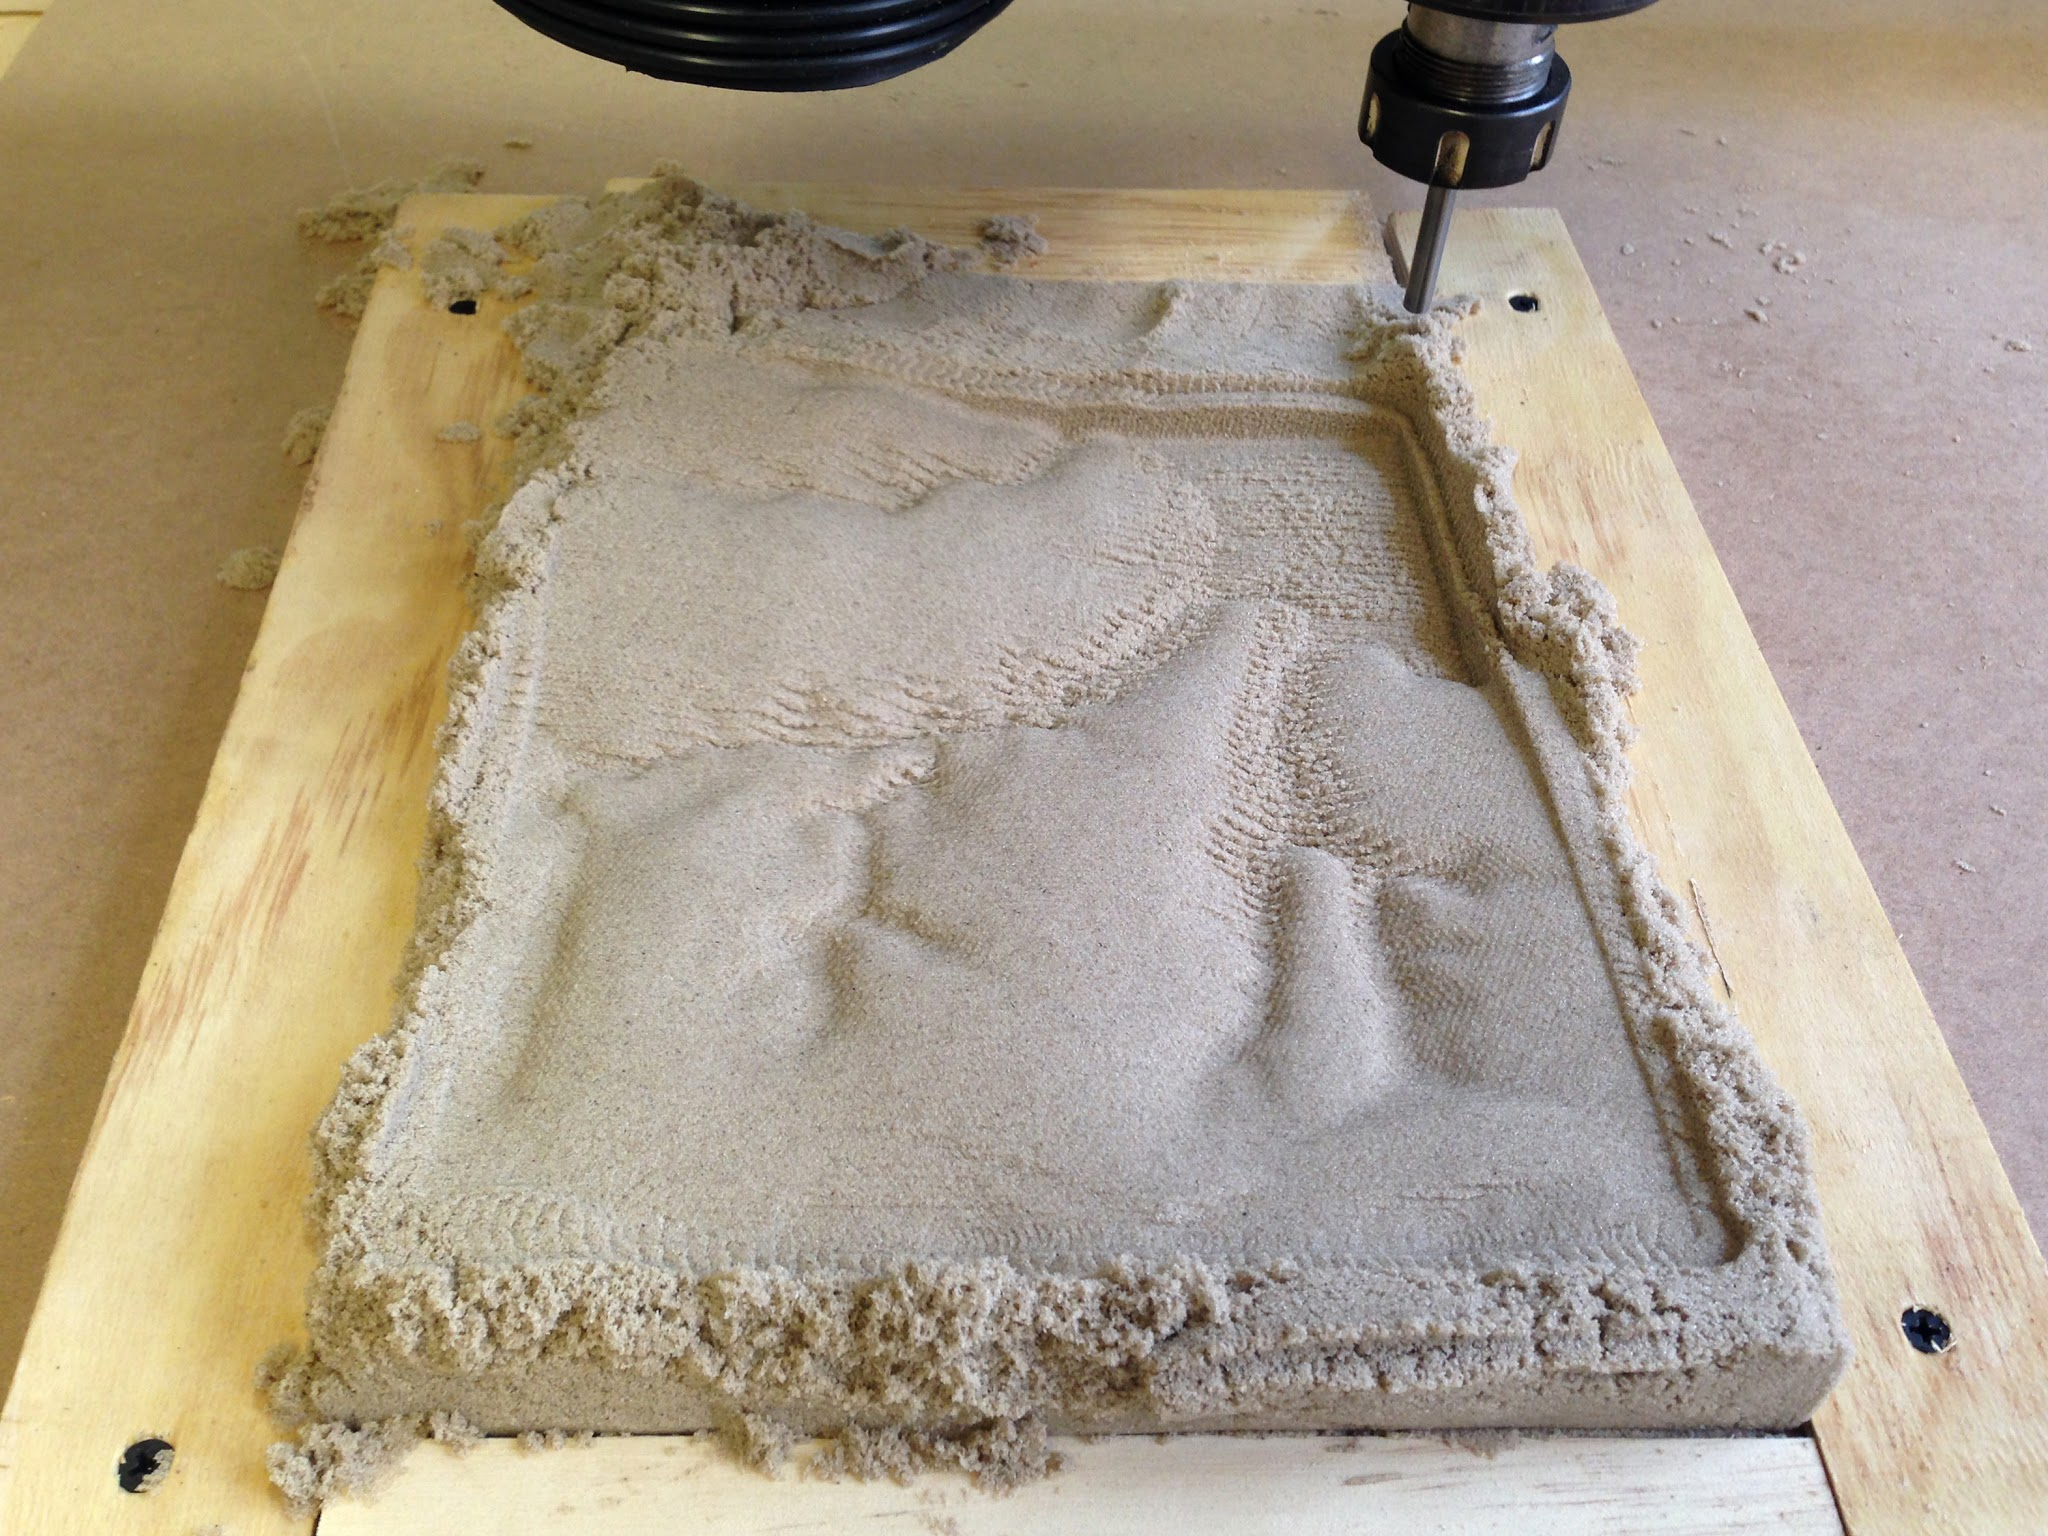
\includegraphics[width=\textwidth]{images/cnc_sand.jpg}
\caption{{\bf Rapid prototyping.}
3-axis CNC fabrication of the evolved landscape in polymer-enriched sand using a plunge cut.}
\label{fig:cnc_sand}
\end{figure}




\section{Results}

\begin{figure}
\centering
%   
\begin{subfigure}[b]{0.3\textwidth}
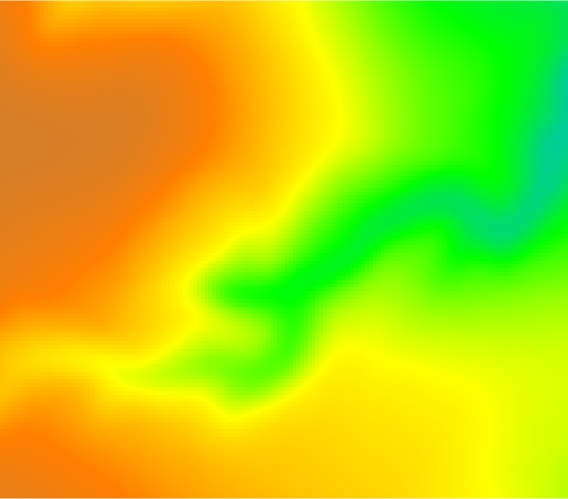
\includegraphics[width=\textwidth]{images/lrwoods_elevation.png}
%[trim={0 0 0 1cm},clip,width=\textwidth]
\label{fig_1_1}
\textbf{a} \\
\end{subfigure}
%
~ %add desired spacing between images, e. g. ~, \quad, \qquad, \hfill etc.
%
\begin{subfigure}[b]{0.3\textwidth}
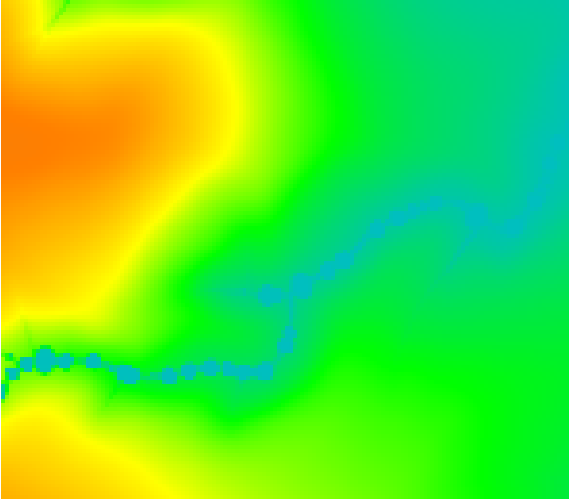
\includegraphics[width=\textwidth]{images/lrwoods_dynamics_flux_5m_30m.png}
\label{fig_1_2}
\textbf{b} \\
\end{subfigure}
%
~ %add desired spacing between images, e. g. ~, \quad, \qquad, \hfill etc.
%
\begin{subfigure}[b]{0.3\textwidth}
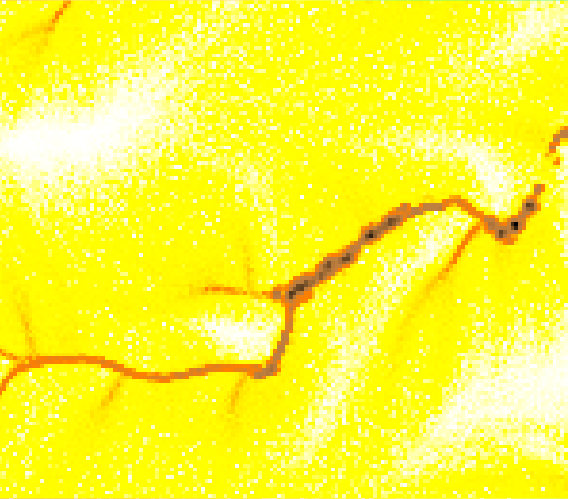
\includegraphics[width=\textwidth]{images/lrwoods_dynamics_erdep_5m_30m_flux.png} % REPLACE IMAGE
\label{fig_1_3}
\textbf{c} \\
\end{subfigure}
%
\caption{{\bf Sediment flux based gully evolution.}
\textbf{a)}
A bare earth digital elevation model of gully in Lake Raleigh Woods, North Carolina derived from lidar data.
\textbf{b)}
The simulated evolution of the gully based on a detachment limited soil erosion regime.
The landscape evolution model was run as a dynamic simulation with 155 mm/hr rainfall intensity for 5 minutes intervals over a 30 min period.
This run of model carved deep pits along the center of the channel.
\textbf{c)}
Simulated sediment flux. 
}
\label{fig_1}
\end{figure}



\begin{figure}
\centering
%   
\begin{subfigure}[b]{0.3\textwidth}
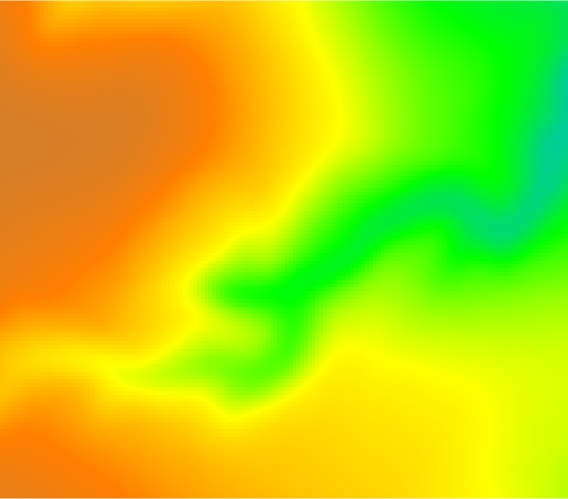
\includegraphics[width=\textwidth]{images/lrwoods_elevation.png}
%[trim={0 0 0 1cm},clip,width=\textwidth]
\label{fig_2_1}
\textbf{a} \\
\end{subfigure}
%
~ %add desired spacing between images, e. g. ~, \quad, \qquad, \hfill etc.
%
\begin{subfigure}[b]{0.3\textwidth}
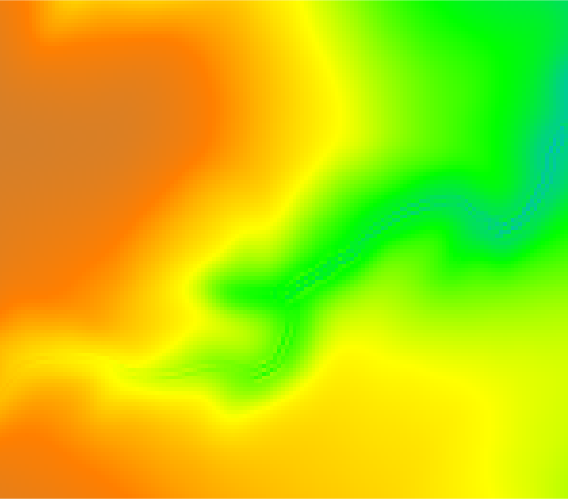
\includegraphics[width=\textwidth]{images/lrwoods_dynamics_erdep_5m_30m.png}
\label{fig_2_2}
\textbf{b} \\
\end{subfigure}
%
~ %add desired spacing between images, e. g. ~, \quad, \qquad, \hfill etc.
%
\begin{subfigure}[b]{0.3\textwidth}
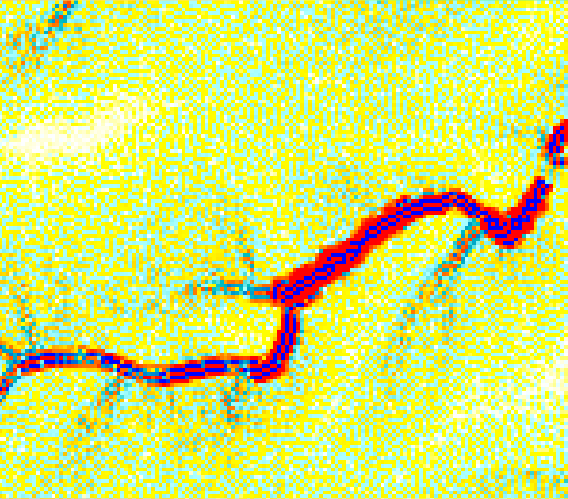
\includegraphics[width=\textwidth]{images/lrwoods_dynamics_erdep_5m_30m_erdep.png} % REPLACE IMAGE
\label{fig_2_3}
\textbf{c} \\
\end{subfigure}
%
\caption{{\bf Erosion - deposition based gully evolution.}
\textbf{a)}
A bare earth digital elevation model of gully in Lake Raleigh Woods, North Carolina derived from lidar data.
\textbf{b)}
The simulated evolution of the gully based on a transport capacity limited  soil erosion regime.
The landscape evolution model was run as a dynamic simulation with 155 mm/hr rainfall intensity for 5 minutes intervals over a 30 min period.
This run of model carved a deeper channel, accumulated deposited sediment along the centerline of the channel, and accumulated deposited sediments along the banks of the channel.
\textbf{c)}
Simulated erosion-deposition. 
}
\label{fig_1}
\end{figure}





\begin{figure}
\centering
%   
\begin{subfigure}[b]{0.4\textwidth}
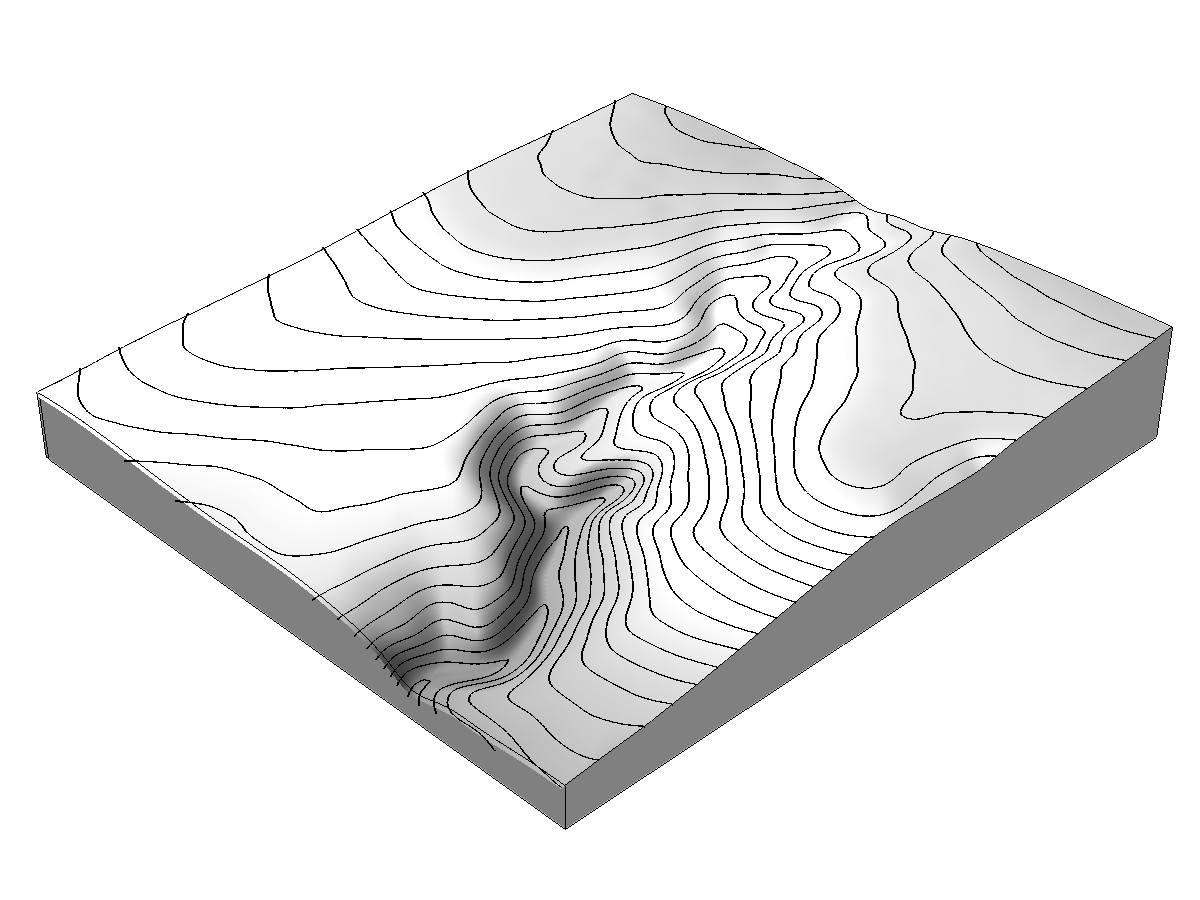
\includegraphics[width=\textwidth]{images/dem.png}
%[trim={0 0 0 1cm},clip,width=\textwidth]
\label{fig_2_1}
\textbf{a} \\
\end{subfigure}
%
~ %add desired spacing between images, e. g. ~, \quad, \qquad, \hfill etc.
%
\begin{subfigure}[b]{0.4\textwidth}
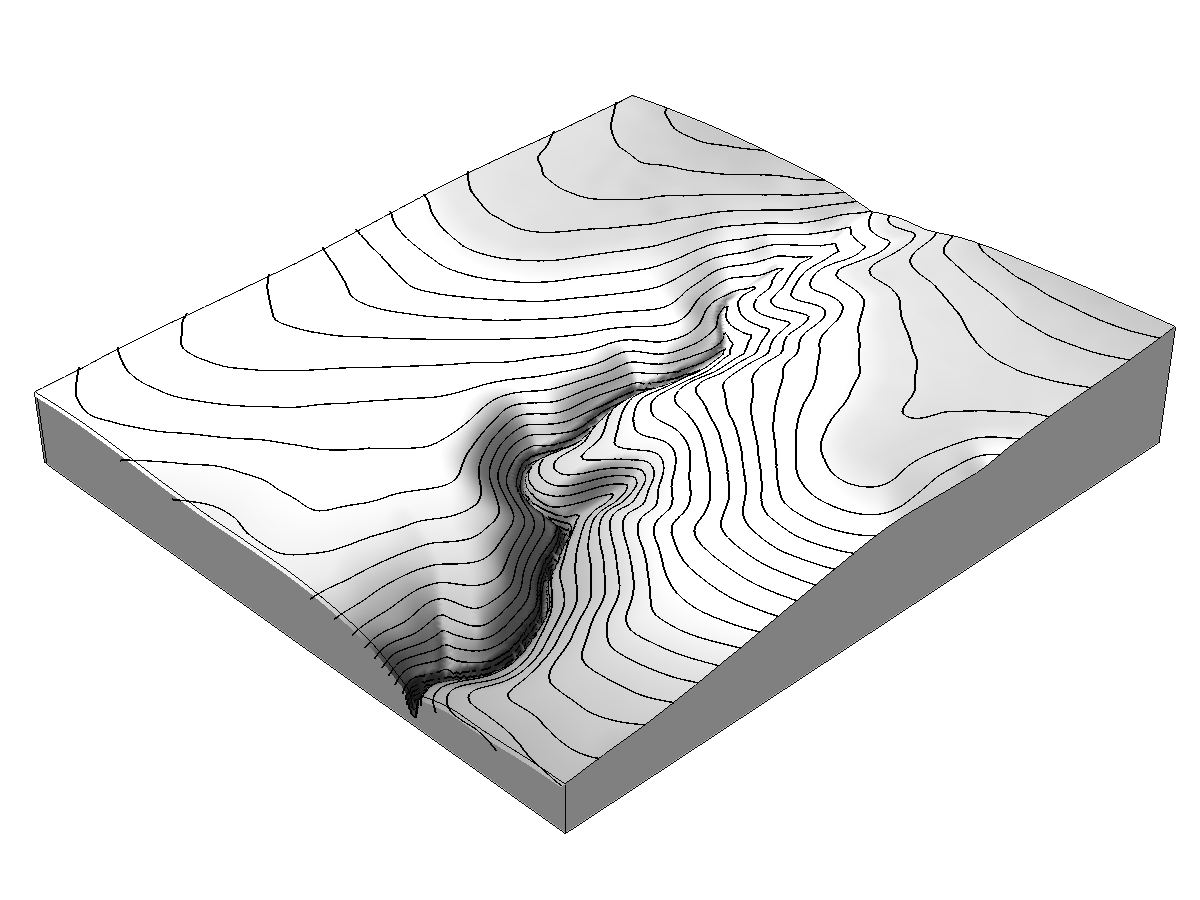
\includegraphics[width=\textwidth]{images/evolved_dem.png}
\label{fig_2_2}
\textbf{b} \\
\end{subfigure}
%
\caption{{\bf Sediment flux based gully evolution.}
\textbf{a)}
A gully in Lake Raleigh Woods, North Carolina.
\textbf{b)}
The simulated evolution of the gully based on a detachment limited soil erosion regime. 
The landscape evolution model was run as a steady state simulation with 155 mm/hr rainfall intensity for 10 minutes to model a 10-year storm event. 
This run of the model carved a deep incision along the centerline of the channel.
}
\label{fig_2}
\end{figure}




\begin{figure}
\centering
%   
\begin{subfigure}[b]{0.4\textwidth}
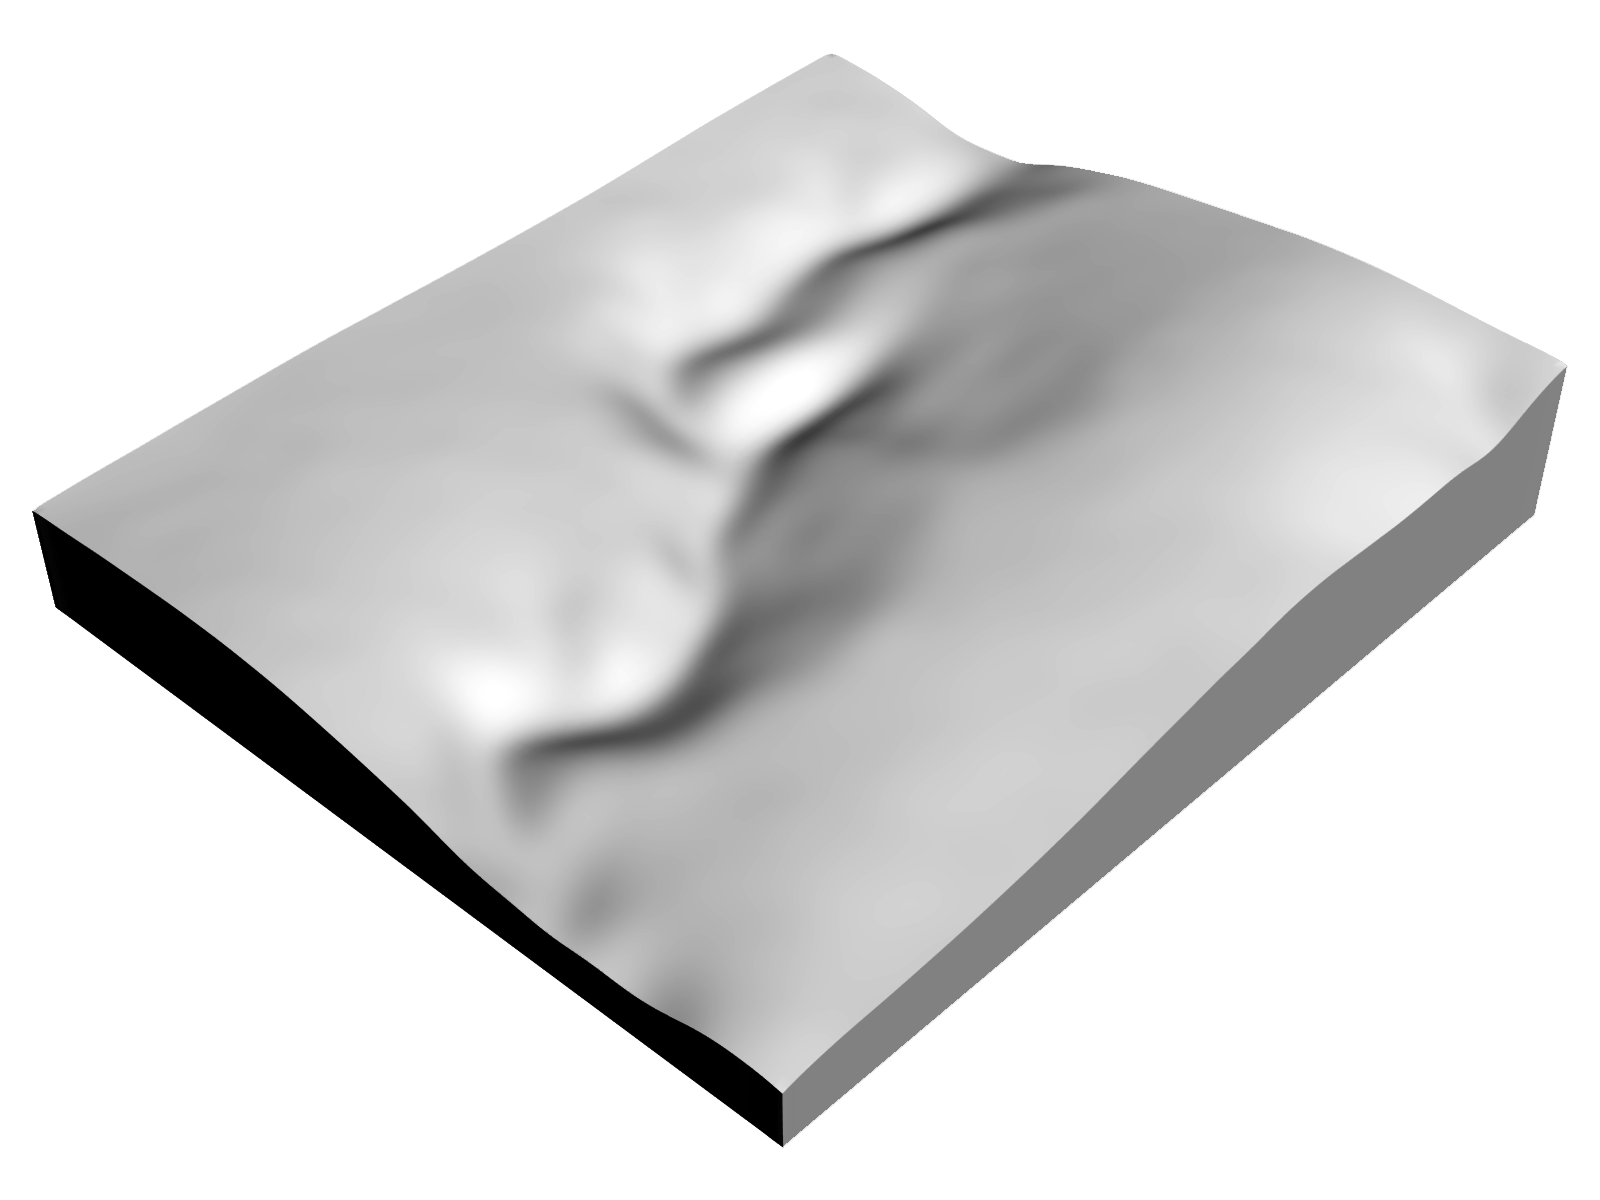
\includegraphics[width=\textwidth]{images/elevation_render.png}
%[trim={0 0 0 1cm},clip,width=\textwidth]
\label{fig_3_1}
\textbf{a} \\
\end{subfigure}
%
~ %add desired spacing between images, e. g. ~, \quad, \qquad, \hfill etc.
%
\begin{subfigure}[b]{0.4\textwidth}
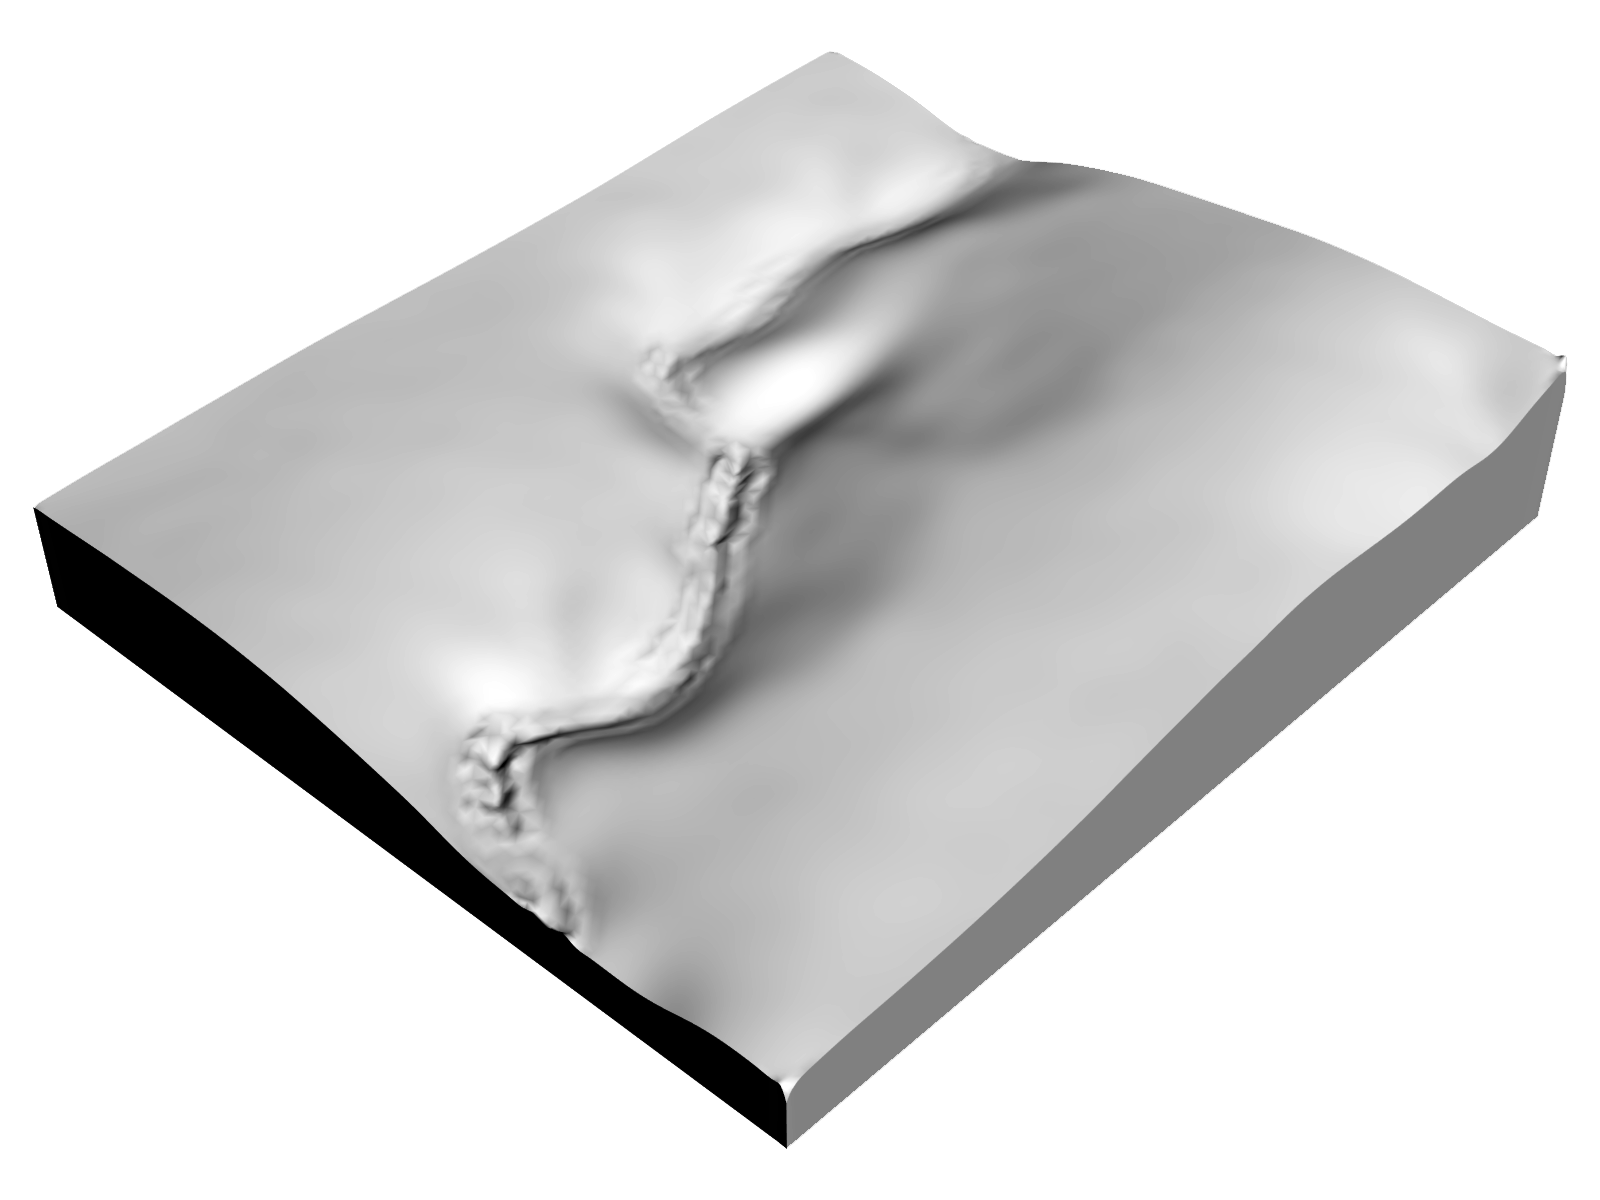
\includegraphics[width=\textwidth]{images/evolved_elevation_render.png}
\label{fig_3_2}
\textbf{b} \\
\end{subfigure}
%
\caption{{\bf Erosion-deposition based gully evolution.}
\textbf{a)}
A gully in Lake Raleigh Woods, North Carolina.
\textbf{b)}
The simulated evolution of the gully based on a transport capacity limited  soil erosion regime.
The landscape evolution model was run as a dynamic simulation with 155 mm/hr rainfall intensity for 5 minutes intervals over a 30 min period.
This run of model carved a deeper channel, accumulated deposited sediment along the centerline of the channel, and accumulated deposited sediments along the banks of the channel.
}
\label{fig_3}
\end{figure}



\section{Discussion}

\subsection{Future work}
\begin{enumerate}
\item Add water and suspended sediment particles to next run
\item Test the model on historical data
\item Test the model with field data
\item Empirically calibrate the parameters
\item Refactor code
\item Develop a GRASS GIS addon
\item Implement as a Tangible Landscape analysis
\item Live, in-situ fabrication in polymer-enriched sand with a robotic arm
\end{enumerate}


\section{Supporting Information}

\subsection{S1 File.}
\label{S1_File}
{\bf Python scripts.}
(ZIP)

\subsection{S2 File.}
\label{S2_File}
{\bf GIS data.}
(ZIP)

% \bibliographystyle{elsarticle-num}
 \bibliographystyle{elsarticle-harv}
% \bibliographystyle{elsarticle-num-names}
% \bibliographystyle{model1a-num-names}
% \bibliographystyle{model1b-num-names}
% \bibliographystyle{model1c-num-names}
% \bibliographystyle{model1-num-names}
% \bibliographystyle{model2-names}
% \bibliographystyle{model3a-num-names}
% \bibliographystyle{model3-num-names}
% \bibliographystyle{model4-names}
% \bibliographystyle{model5-names}
% \bibliographystyle{model6-num-names}

\bibliography{landscape_evolution.bib}


\end{document}

